\documentclass[12pt, a4paper]{article}
\usepackage[british]{babel}
\usepackage[utf8]{inputenc}
\usepackage{amsmath}
\usepackage{amssymb}
\usepackage{amsthm}
\usepackage{booktabs}
\usepackage{pgfplots}
\usepackage{relsize}
\usepackage{subfig}
%\usepackage{epstopdf}
\usepackage{graphicx}
\usepackage[en-US]{datetime2}
\usepackage[font=small, textfont=sl]{caption}
\usepackage[hidelinks]{hyperref}
\graphicspath{{img/}}
\pgfplotsset{compat=newest, every axis/.append style = {font=\relsize{-2}}}

\theoremstyle{definition}
\newtheorem{ipotesi}{Assumption}

\theoremstyle{plain}
\newtheorem{lemma}{Lemma}

\theoremstyle{plain}
\newtheorem{teor}{Theorem}

\theoremstyle{definition}
\newtheorem*{remark}{Remark}

\title{\textbf{Discontinuous Galerkin Finite Element approximations of elliptic 
problems on polyhedral grids}}
\author{Andrea Vescovini\\[1cm]{\small Supervisor: Prof. P. Antonietti}}
\DTMlangsetup{showdayofmonth=false}
\date{\today}
%\institute[Polimi]{Politecnico di Milano}
%%%%%%%%%%%%%%%%%%%%%%%%%%%%%%%%%%%%%%%%%%%%%%%%%%%%%%%%%%%%%%%%%%%%%%%%%%

\begin{document}
\maketitle
\centerline{Politecnico di Milano}
\newpage
\begin{abstract}
	The main goal of this project is to implement a Discontinuous Galerkin (DG) 
	finite element method for solving a three-dimensional Poisson problem with 
	Dirichlet boundary conditions, employing a general polyhedral mesh.\\
	Discontinuous Galerkin methods have shown to be very flexible and have been 
	successfully 
	applied to hyperbolic, elliptic and parabolic problems arising from many 
	different fields of application.
	Moreover one of the main advantages with respect to the continuous 
	framework is the possibility of handling meshes with hanging nodes and made 
	of general-shaped elements without any difficulty. Meshes made of 
	general polyhedral elements can be useful in many problems, especially when 
	we have to deal with domains that present small details or microstructures; 
	these features would need too many ``classical" tetrahedral/hexahedral 
	elements to be described and so too many degrees of freedom.\\
	In Section~\ref{sec:DG} we recall the main results about standard DG 
	methods, then in Subsection~\ref{sec:poly} we develop the theory in order 
	to 
	handle polyhedral grids. Afterwards in Section~\ref{sec:imp} we explain our 
	main choices for the algorithm implementation and in Section~\ref{sec:res} 
	we present some numerical results conforming to the theoretical estimates.
\end{abstract}
\newpage
\phantomsection
\tableofcontents
\newpage

%%%%%%%%%%%%%%%%%%%%%%%%%%%%%%%%%%%%%%%%%%%%%%%%%%%%%%%%%%%%%%%%%%%%%%%%%

%\section*{Introduction}
%Introduzione sì o introduzione no?

\section[Discontinuous Galerkin finite element methods]{Discontinuous Galerkin 
finite element\\methods}\label{sec:DG}
In this section we follow mainly chapter 2 of \cite{riviere} and chapter 11 of \cite{quart}.
\subsection{Model problem}
Let us consider a Poisson problem with Dirichlet boundary conditions
\begin{align} \label{eq:poisson}
	-\Delta u = f & \mbox{ in } \Omega\\
			u = g & \mbox{ on } \partial \Omega
\end{align}
where $\Omega \subset \mathbb{R}^3$ is a convex bounded polyhedral domain with 
a Lipschitz boundary $\partial \Omega$, the source $f$ belongs to $L^2(\Omega)$ 
and the Dirichlet datum $g$ belongs to $H^{1/2}(\partial \Omega)$.
The usual weak formulation is:\\
Find $u \in H^1(\Omega)$ such that $u = \tilde{u} + R_g$, with $\tilde{u} \in H^1_0(\Omega)$ such that:
\begin{equation} \label{eq:wform}
	\int_\Omega \nabla u \cdot \nabla v
	= \int_\Omega fv - \int_\Omega \nabla R_g \cdot \nabla v \quad \forall v 
	\in H^1_0(\Omega),
\end{equation}
and $R_g \in H^1(\Omega)$ is a lifting of $g$, i.e. $R_g|_{\partial \Omega} = g$.\\
Discontinuous Galerkin methods make use of a variational formulation different 
from the usual one so we have to introduce new spaces in which we will look for 
the solution.
%%%%%%%%%%%%%%%%%%%%%%%%%%%%%%%%%%%%%%%%%%%%%%%%%%%%%%%%%%%%%%%%%%%%%%%%%%%%%%%%
\subsection{Broken Sobolev spaces}
Let $\mathcal{T}$ be a subdivision of $\Omega$ into disjoint open tetrahedral elements $\kappa$ such that $\bar{\Omega} = \bigcup\limits_{\kappa \in \mathcal{T}} \bar{\kappa}$, let $h_\kappa$ be the diameter of the element $\kappa$ i.e. $h_\kappa = \min\limits_{x, y \in \kappa} |x-y|$ and let $\rho_\kappa$ be the maximum diameter of a ball inscribed in $\kappa$. For the moment we assume $\mathcal{T}$ to be regular, i.e. that $\exists C > 0$ such that:
\begin{equation*}
	\frac{h_\kappa}{\rho_\kappa} < C \quad \forall \kappa \in \mathcal{T}.
\end{equation*}
We define for every real number $s>0$ the broken Sobolev space:
\begin{equation*}
	H^s(\mathcal{T}) = \{ v \in L^2(\Omega) : v|_\kappa \in H^s(\kappa) \quad 
	\forall \kappa \in \mathcal{T} \},
\end{equation*}
with the norm:
\begin{equation*}
	|\!|\!|v|\!|\!|_{H^s(\mathcal{T})} = \bigg( \sum_{\kappa \in \mathcal{T}} |\!|v|\!|_{H^s(\kappa)}^2 \bigg)^{1/2}.
\end{equation*}
By extension $L^2(\mathcal{T})$ can be seen as $H^0(\mathcal{T})$. Moreover it holds that:
\begin{equation*}
	H^s(\Omega) \subset H^s(\mathcal{T}) \quad \text{ and } \quad 
	H^{s+1}(\mathcal{T}) \subset H^s(\mathcal{T}).
\end{equation*}
We denote by $\Gamma_h$ the set of interior faces, by $\Gamma_D$ the set of 
faces that are on the boundary $\partial \Omega$ and we define $\Gamma = 
\Gamma_h \cup \Gamma_D$. Here a face is intended to be the (open) intersection 
of the closure of two neighbouring elements $\kappa^\pm \in \mathcal{T}$. For 
every face $e \in \Gamma_h$ there exist two elements 
$\kappa^+$ and $\kappa^-$ that share it and they both have their outward normal 
$\mathbf{n}^+$ and $\mathbf{n}^-$.\\
Since every function $v$ of $H^s(\mathcal{T}), \; s \geq 1$ is well defined 
along any side of every $\kappa$, if $e \in \Gamma_h$ there are two different 
traces of $v$ along $e$ and we denote them by $v^+$ and $v^-$.
It will be useful to introduce jumps and average of these traces so we can 
define:
\begin{align}
	[v] = v^+ \mathbf{n}^+ + v^- \mathbf{n}^-,
	&\quad [\![ \mathbf{v} ]\!] = \mathbf{v}^+ \cdot \mathbf{n}^+ + \mathbf{v}^- \cdot \mathbf{n}^-, \label{eq:jump} \\
	\{v\} = \frac{1}{2} (v^+ + v^-) ,
	& \quad \{\!\!\{ \mathbf{v} \}\!\!\} = \frac{1}{2} (\mathbf{v}^+ +\mathbf{v}^-), \label{eq:aver}
\end{align}
that can be extended to $e \in \Gamma_D$ through:
\begin{equation} \label{eq:jupsandaverdir}
	[v] = v \mathbf{n},
	\quad [\![ \mathbf{v} ]\!] = \mathbf{v} \cdot \mathbf{n},
	\quad \{v\} = v,
	\quad \{\!\!\{ \mathbf{v} \}\!\!\} = \mathbf{v}.
\end{equation}
\begin{remark}
	Notice that the above definitions are independent of which element is 
	called ``$^+$" and which ``$^-$".
\end{remark}
%%%%%%%%%%%%%%%%%%%%%%%%%%%%%%%%%%%%%%%%%%%%%%%%%%%%%%%%%%%%%%%%%%%%%%%%%%%%%%
\subsection{Variational formulation}
In what follows we assume that the weak solution $u$ of the Poisson problem~ \eqref{eq:wform} belongs to $H^s(\mathcal{T})$ with $s > 3/2$, so that the following calculations will be meaningful.\\
Integrating \eqref{eq:poisson} by parts we can obtain:
\begin{equation} \label{eq:green}
	\sum_{\kappa \in \mathcal{T}} \int_\kappa -\Delta u \; v
	= \sum_{\kappa \in \mathcal{T}} \bigg( \int_\kappa \nabla u \cdot \nabla v
	- \int_{\partial \kappa} v \nabla u \cdot \mathbf{n} \bigg) \quad \forall v 
	\in H^s(\mathcal{T}).
\end{equation}
With some manipulations we can see that:
\begin{equation} \label{eq:jumps}
\begin{split}
	\sum_{\kappa \in \mathcal{T}} \int_{\partial \kappa} v \nabla u \cdot \mathbf{n} &= \sum_{e \in \Gamma} \int_e (v^+ \nabla u^+ \cdot \mathbf{n}^+ + v^- \nabla u^- \cdot \mathbf{n}^- )\\
	&= \sum_{e \in \Gamma} \int_e ([v] \cdot \{\!\!\{ \nabla u \}\!\!\} + [\![ 
	\nabla u ]\!] \{v\} ) \quad \forall v \in H^s(\mathcal{T}).
\end{split}
\end{equation}
Then inserting~\eqref{eq:jumps} into~\eqref{eq:green} we can obtain that the solution of the Poisson problem~\eqref{eq:poisson} is $u \in H^s(\mathcal{T})$ such that:
\begin{equation} \label{eq:firstform}
	\sum_{\kappa \in \mathcal{T}} \int_\kappa \nabla u \cdot \nabla v -
	\sum_{e \in \Gamma} \int_e ([v] \cdot \{\!\!\{ \nabla u \}\!\!\} + [\![ \nabla u ]\!] \{v\} ) =
	\sum_{\kappa \in \mathcal{T}} \int_\kappa fv \quad \forall v \in 
	H^s(\mathcal{T}).
\end{equation}
At this point we have to observe that since the domain $\Omega$ is convex, the 
exact solution $u \in H^2(\Omega)$, and then $[\![\nabla u]\!] = 0$ and $[u] = 
0$ on every internal face $e \in \Gamma_h$. For this reason 
in~\eqref{eq:firstform} the term~$[\![ \nabla u ]\!] \{v\}$ is null and we can 
add on the left hand side two tunable terms:
\begin{equation*}
	\epsilon \sum_{e \in \Gamma_h} \int_e [u] \cdot \{\!\!\{ \nabla v \}\!\!\},
\end{equation*}
\begin{equation*}
	\sum_{e \in \Gamma_h} \gamma_e \int_e [u] \cdot [v], \quad \gamma_e = 
	\frac{\sigma_e}{|e|^\beta}
\end{equation*}
where $\epsilon = \{-1, 0, 1\}$ is a parameter that will affect the symmetry of 
the formulation, $|e|$ is the two-dimensional measure of the face $e$, 
$\sigma_e$ and $\beta$ are two parameters that will be specified later and will 
be important for the well~posedness of the problem.\\
Finally we impose the Dirichlet boundary condition in a weak sense, as it is 
more natural for a DG method, so we add on the left hand side:
\begin{equation*}
	\epsilon \sum_{e \in \Gamma_D} \int_e (u-g) \nabla v \cdot \mathbf{n}
	+ \sum_{e \in \Gamma_D} \gamma_e \int_e (u-g)v.
\end{equation*}
We have obtained the general DG variational formulation:\\
Find $u \in H^s(\mathcal{T}), s>3/2$, such that:
\begin{multline*}
	\sum_{\kappa \in \mathcal{T}} \int_\kappa \nabla u \cdot \nabla v 
	-\sum_{e \in \Gamma} \bigg( \int_e [v] \cdot \{\!\!\{ \nabla u \}\!\!\}
	-\epsilon \int_e [u] \cdot \{\!\!\{ \nabla v \}\!\!\}
	- \gamma_e \int_e [u] \cdot [v] \bigg)\\
	= \sum_{\kappa \in \mathcal{T}} \int_\kappa fv
	+ \sum_{e \in \Gamma_D} \bigg( \epsilon \int_e g \nabla v \cdot \mathbf{n}
	+ \gamma_e \int_e gv \bigg) \quad \forall v \in H^s(\mathcal{T}).
\end{multline*}
Viceversa it can be proved (see \cite{riviere}) that if the solution 
$u$ of 
\eqref{eq:dgvarform} belongs to $H^1(\Omega) \cap H^s(\mathcal{T})$, then $u$ 
is the solution of the Poisson problem \eqref{eq:poisson}.\\
We can introduce the bilinear form $a_\epsilon:~H^s(\mathcal{T})~\times~H^s(\mathcal{T})~\rightarrow~\mathbb{R}$:
\begin{equation*}
a_\epsilon(u, v) = \sum_{\kappa \in \mathcal{T}} \int_\kappa \nabla u \cdot \nabla v
-\sum_{e \in \Gamma} \bigg( \int_e [v] \cdot \{\!\!\{ \nabla u \}\!\!\}
-\epsilon \int_e [u] \cdot \{\!\!\{ \nabla v \}\!\!\}
- \gamma_e \int_e [u]\cdot[v] \bigg)
\end{equation*}
and the functional $F_\epsilon:~H^s(\mathcal{T})~\rightarrow~\mathbb{R}$:
\begin{equation*}
	F_\epsilon(v) = \sum_{\kappa \in \mathcal{T}} \int_\kappa fv
	+ \sum_{e \in \Gamma_D} \bigg( \epsilon \int_e g \nabla v \cdot \mathbf{n}
	+ \gamma_e \int_e gv \bigg),
\end{equation*}
so that we can rewrite the variational formulation in a compact fashion:\\
Find $u \in H^s(\mathcal{T}), \; s>3/2$, such that:
\begin{equation} \label{eq:dgvarform}
	a_\epsilon(u, v) = F_\epsilon(v) \quad \forall v \in H^s(\mathcal{T}).
\end{equation}
%%%%%%%%%%%%%%%%%%%%%%%%%%%%%%%%%%%%%%%%%%%%%%%%%%%%%%%%%%%%%%%%%%%%%%%%%%%
\subsection{Discrete formulation}
We introduce now the finite dimensional subspace of $H^s(\mathcal{T})$, $s>3/2$:
\begin{equation} \label{eq:dgspace}
	\mathcal{D}_r(\mathcal{T}) = \{ v \in L^2(\Omega) : v|_\kappa \in 
	\mathbb{P}_r(\kappa) \quad \forall \kappa \in \mathcal{T}  \},
\end{equation}
where $\mathbb{P}_r(\kappa)$ denotes the space of polynomials of total degree 
less then or equal to $r$ over the element $\kappa$. We endow it with the so 
called \textit{energy norm}:
\begin{equation*}
	|\!|v_h|\!|_{DG} = \bigg( |\!|\nabla v_h|\!|^2_{L^2(\mathcal{T})} + \sum_{e \in \Gamma} \gamma_e \int_e [v_h]^2 \bigg)^{1/2}.
\end{equation*}
It is easy to see that it is a norm if $\gamma_e > 0 \quad \forall e \in 
\Gamma$. The general DG finite element formulation is:\\
Find $u_h \in \mathcal{D}_r(\mathcal{T})$ such that:
\begin{equation} \label{eq:dgfemform}
	a_\epsilon(u_h, v_h) = F_\epsilon(v_h) \quad \forall v_h \in 
	\mathcal{D}_r(\mathcal{T}).
\end{equation}
This kind of formulation is called \textit{Interior Penalty} (IP) and as briefly mentioned before the parameter $\epsilon$ can influence the symmetry:
\begin{itemize}
\item
If $\epsilon = -1$ the method is called \textit{Symmetric Interior Penalty 
Galerkin} (SIPG), indeed in the bilinear form becomes symmetrical because the 
two terms involving jumps and averages appear with the same sign. Introduced by 
Arnold \cite{arn82} and Wheeler \cite{whe78}.
\item
If  $\epsilon = +1$ the method is called \textit{Non-symmetric Interior Penalty 
Galerkin} (NIPG), for an opposite reason. Introduced by Rivière, Wheeler 
and Girault \cite{rwg}.
\item
If $\epsilon = 0$ the method is called \textit{Incomplete Interior Penalty 
Galerkin} (IIPG) Introduced by Dawson, Sun and Wheeler \cite{dsw}.
\end{itemize}
%%%%%%%%%%%%%%%%%%%%%%%%%%%%%%%%%%%%%%%%%%%%%%%%%%%%%%%%%%%%%%%%%%%%%%%%%%
\subsection{Consistency}
We show the consistency of the discrete formulation~\eqref{eq:dgfemform} 
specifying the variational formulation~\eqref{eq:dgvarform} for test 
functions of the space $\mathcal{D}_r(\mathcal{T})$:
\begin{equation*}
	a_\epsilon(u, v_h) = F_\epsilon(v_h) \quad v_h \in 
	\mathcal{D}_r(\mathcal{T}).
\end{equation*}
We subtract~\eqref{eq:dgfemform} to the above formulation and we get error 
$u-u_h$ satisfies the following \textit{Galerkin orthogonality} property:
\begin{equation*}
		a_\epsilon(u - u_h, v_h) = 0 \quad v_h \in 
		\mathcal{D}_r(\mathcal{T}).
\end{equation*}
%%%%%%%%%%%%%%%%%%%%%%%%%%%%%%%%%%%%%%%%%%%%%%%%%%%%%%%%%%%%%%%%%%%%%%%%%%%
\subsection{Well posedness}
In order to prove the well posedness of \eqref{eq:dgfemform} we have to show 
coercivity and continuity of the bilinear form and continuity of the functional 
with respect to the norm $||\cdot||_{DG}$, then apply the Lax-Milgram lemma.\\
We will use the following inverse trace inequality for polynomials 
(\cite{riviere}, p.~23):
\begin{equation} \label{eq:trineq}
	|\!|v|\!|_{L^2(e)} \leq \frac{\bar{C}}{\sqrt{h_\kappa}} 
	|\!|v|\!|_{L^2(\kappa)} \quad \forall e \subset \partial \kappa \quad 
	\forall 
	v \in \mathbb{P}_r(\kappa).
\end{equation}
%%%%%%%%%%%%%%%%%%%%%%%%%%%%%%%%%%%%%%%%%%%%%%%%%%%%%%%%%%%%%%%%%%%%%%%%%%
\subsubsection{Coercivity}
We have to show that $\exists \alpha > 0 $ such that:
\begin{equation*}
a_\epsilon(u_h, u_h) = |\!|u_h|\!|^2_{DG} + (\epsilon - 1) \sum_{e \in \Gamma} \int_e [u_h] \cdot \{\!\!\{ \nabla u_h \}\!\!\} \geq \alpha |\!|u_h|\!|^2_{DG}.
\end{equation*}
If $\epsilon = 1$ we get immediately the coercivity with a coercivity constant $\alpha = 1$.
If $\epsilon = \{0,-1\}$ more care is needed: using Cauchy-Schwarz's inequality 
and Young's inequality we obtain $\forall \delta > 0$:
\begin{equation} \label{pas:young}
\bigg| \sum_{e \in \Gamma} \int_e [u_h] \cdot \{\!\!\{ \nabla u_h \}\!\!\} \bigg| \leq
\frac{\delta}{2} \sum_{e \in \Gamma} \bigg( \frac{1}{\gamma_e} \bigg)  \big|\!\big| \{\!\!\{ \nabla u_h \}\!\!\} \big|\!\big|^2_{L^2(e)}
+ \frac{1}{2\delta} \bigg|\!\bigg| \sqrt{\gamma_e} [u_h] \bigg|\!\bigg|^2_{L^2(\Gamma)}
\end{equation}
Then we observe that:
\begin{equation*}
\big|\!\big| \{\!\!\{ \nabla u_h \}\!\!\} \big|\!\big|^2_{L^2(e)} \leq
\begin{cases}
\big|\!\big| \nabla u_h \big|\!\big|^2_{L^2(e)}, & \text{if } e \in \Gamma_D\\
\frac{1}{4} \big( \big|\!\big| \nabla u_h|_{\kappa^+} \big|\!\big|^2_{L^2(e)} + \big|\!\big| \nabla u_h|_{\kappa^-} \big|\!\big|^2_{L^2(e)} \big), & \text{if } e \in \Gamma_h
\end{cases}
\end{equation*}
and use the inverse trace inequality \eqref{eq:trineq}, to obtain:
\begin{equation*}
\big|\!\big| \nabla u_h \big|\!\big|^2_{L^2(e)} \leq \frac{\bar{C}^2}{h_\kappa} \big|\!\big| \nabla u_h \big|\!\big|^2_{L^2(\kappa)}.
\end{equation*}
Now we exploit the fact that trivially $|e| < h_\kappa^{d-1} \quad \forall e 
\subset \partial \kappa$, where $d$ is the dimension in which we are working, 
i.e. $d = 3$:
\begin{multline} \label{pas:invineq}
\sum_{e \in \Gamma} \bigg( \frac{|e|^\beta}{\sigma_e} \bigg)  \big|\!\big| \{\!\!\{ \nabla u_h \}\!\!\} \big|\!\big|^2_{L^2(e)}
\leq \sum_{e \in \Gamma_h} \frac{\bar{C}^2}{4\sigma_e} \bigg( h_{\kappa^+}^{2\beta - 1} \big|\!\big| \nabla u_h \big|\!\big|^2_{L^2(\kappa^+)} + h_{\kappa^-}^{2\beta - 1} \big|\!\big| \nabla u_h \big|\!\big|^2_{L^2(\kappa^-)} \bigg)\\
+ \sum_{e \in \Gamma_D} \frac{\bar{C}^2}{\sigma_e} h_\kappa^{2\beta - 1} \big|\!\big| \nabla u_h \big|\!\big|^2_{L^2(\kappa)}
\leq \sum_{\kappa \in \mathcal{T}} \sum_{e \in \partial \kappa} \frac{\bar{C}^2}{\sigma_e} \big|\!\big| \nabla u_h \big|\!\big|^2_{L^2(\kappa)}
\leq \frac{n^*\bar{C}^2}{\sigma^*} \big|\!\big| \nabla u_h \big|\!\big|^2_{L^2(\mathcal{T})}.
\end{multline}
We assume that $2\beta - 1 \geq 0$, we suppose, without loss of generality, 
that 
$h~=~\min\limits_{\kappa \in \mathcal{T}} h_\kappa~<~1$, we define $\sigma^* = 
\min\limits_{e \in \Gamma} \sigma_e$ and $n^*$ to be the number of faces for 
every element. Putting together \eqref{pas:young} and \eqref{pas:invineq} we 
obtain:
\begin{equation*}
\begin{split}
a_\epsilon(u_h, u_h) &\geq \big(1 - \frac{n^*\delta\bar{C}^2}{2\sigma^*} (1-\epsilon)\big) \big|\!\big| \nabla u_h \big|\!\big|^2_{L^2(\mathcal{T})}
+ \big(1 - \frac{1}{2\delta} \big) \bigg|\!\bigg| \sqrt{\gamma_e} [u_h] \bigg|\!\bigg|^2_{L^2(\Gamma)}\\
&\geq \min\bigg\{1 - \frac{n^*\delta\bar{C}^2}{2\sigma^*} (1-\epsilon) , 1 - \frac{1-\epsilon}{2\delta}\bigg\} |\!|u_h|\!|^2_{DG}
\end{split}
\end{equation*}
Choosing for example $\delta = 1$ for $\epsilon = 0$ and  $\delta = 1/2$ for 
$\epsilon = -1 $ we need then $\sigma^* > (n^*\bar{C}^2)/2$ in order to get the 
coercivity constant $\alpha > 0$.
%%%%%%%%%%%%%%%%%%%%%%%%%%%%%%%%%%%%%%%%%%%%%%%%%%%%%%%%%%%%%%%%%%%%%%%%%%
\subsubsection{Continuity}
We have to show that $\exists M_1 > 0$ such that:
\begin{equation*}
	|a_\epsilon(u_h, v_h)| \leq M_1 |\!|u_h|\!|_{DG} |\!|v_h|\!|_{DG} \quad 
	\forall u_h, v_h \in \mathcal{D}_r(\mathcal{T})
\end{equation*}
and that $\exists M_2 > 0$ such that:
\begin{equation*}
	|F_\epsilon(v_h)| \leq M_2 |\!|v_h|\!|_{DG} \quad \forall v_h \in 
	\mathcal{D}_r(\mathcal{T}).
\end{equation*}
The proof follows easily from standard arguments; indeed exploiting triangular inequality and Cauchy-Schwarz's inequality we can obtain very straight forward the required bounds for the first and last term of $a_\epsilon(u, v)$. For the second and third term we just have to use smartly Cauchy-Schwarz and then apply the trace inequality \eqref{eq:trineq} like for the coercivity.\\
We can proceed analogously for $F_\epsilon(v)$.
%%%%%%%%%%%%%%%%%%%%%%%%%%%%%%%%%%%%%%%%%%%%%%%%%%%%%%%%%%%%%%%%%%%%%%%%%%
\subsubsection{Existence and uniqueness}
Finally we have that:
\begin{itemize}
	\item always for NIPG,
	\item if $\beta \geq 1/2$ and $\sigma^*$ is greater enough for SIPG and 
	IIPG,
\end{itemize}
then Lax-Milgram lemma holds, so the solution $u_h$ of \eqref{eq:dgfemform} 
exists and is unique, moreover:\\
\begin{equation*}
	|\!|u_h|\!|_{DG} \leq \frac{M_2}{\alpha},
\end{equation*}
where $M_2$ is the continuity constant of $F_\epsilon(v_h)$ and $\alpha$ is the 
coercivity constant of $a_\epsilon(u_h,v_h)$ and they depend on $f$, $g$, 
$\bar{C}$ and the polynomial approximation degree $r \geq 1$.
%%%%%%%%%%%%%%%%%%%%%%%%%%%%%%%%%%%%%%%%%%%%%%%%%%%%%%%%%%%%%%%%%%%%%%%%%%%
\subsection{Error analysis}
We quote from \cite{riviere} error bounds both in the $DG$-norm and in the $L^2$-norm.
\begin{teor} \label{teo:errdg}
	Assume that the exact solution to the problem~\eqref{eq:wform} belongs to 
	$H^k(\mathcal{T}), \; k>3/2$. Assume also $\beta = 1/2$ and that the 
	penalty parameter $\sigma_e$ is large enough for the SIPG and IIPG methods. 
	Then $\exists C>0$ independent of~$h$, but dependent on $r \geq 1$, such 
	that:
	\begin{equation*}
		|\!| u -u_h |\!|_{DG} \leq h^{s-1} |\!|\!|u|\!|\!|_{H^k(\mathcal{T})}.
	\end{equation*}
	where $s = \min \{r+1, k\}$.
\end{teor}
\begin{teor}
	Assume that theorem~\ref{teo:errdg} holds. Then for the SIPG method 
	$\exists C>0$ independent of $h$, but dependent on $r \geq 1$, such that:
	\begin{equation*}
		|\!| u-u_h |\!|_{L^2(\Omega)} \leq C h^{s} |\!|\!|u|\!|\!|_{H^k(\mathcal{T})},
	\end{equation*}
	while for both th NIPG and IIPG methods the following suboptimal estimate holds:
	\begin{equation*}
				|\!| u-u_h |\!|_{L^2(\Omega)} \leq C h^{s-1} 
				|\!|\!|u|\!|\!|_{H^k(\mathcal{T})}.
	\end{equation*}
\end{teor}
It has been proved (see \cite{ayuso}) that for NIPG and IIPG convergence rates 
are 
optimal if the 
polynomial degree is odd and suboptimal if it is even.
%%%%%%%%%%%%%%%%%%%%%%%%%%%%%%%%%%%%%%%%%%%%%%%%%%%%%%%%%%%%%%%%%%%%%%%%%%%
\subsection{Extension to polyhedral grids}\label{sec:poly}
In this subsection we extend the previous analysis to grids consisting of 
general polyhedra, following mainly \cite{multigrid} and \cite{hpmet}.
\subsubsection{Grid assumptions}
Suppose that now $\mathcal{T}$ is a partition of the computational domain 
$\Omega$ into disjoint open polyhedral elements $\kappa$, such that 
$\bar{\Omega} = \bigcup_{\kappa \in \mathcal{T}} \bar{\kappa}$. In order to 
allow the presence of hanging nodes/edges, we define the \textit{interfaces} of 
$\mathcal{T}$  as the intersection of the $(d-1)$-dimensional facets of 
neighbouring elements. Then, being us in $d=3$, we assume that each interface 
of an element $\kappa \in \mathcal{T}$ may be subdivided by a set of co-planar 
triangles. So with \textit{face} we refer to a $(d-1)$-dimensional simplex 
(i.e. a triangle in $d=3$), which forms part of an interface of an element 
$\kappa \in \mathcal{T}$; this means that each interface has a 
sub-triangulation into faces. As before with $\Gamma_h$ we denote the union of 
all open faces of the mesh interior to $\Omega$ and with $\Gamma_D$ the union 
of all open faces of the mesh contained in the boundary $\partial \Omega$; then 
$\Gamma = \Gamma_h \cup \Gamma_D$.\\
We need now some assumptions on the mesh $\mathcal{T}$:
\begin{ipotesi} \label{ipo:ipo1}
	Given $\kappa \in \mathcal{T}$, there exists a set of non-overlapping (not 
	necessarily shape-regular) three-dimensional simplices $T_j \subset \kappa, 
	\; j = 1,\dots, n_\kappa$, such that for any face $e \subset \partial 
	\kappa$, $\bar{e} = \partial \bar{\kappa} \cap \partial \bar{T_j}$, for 
	some $j$,
	\begin{equation*}
		\cup_{j = 1}^{n_\kappa} \bar{T_k} \subseteq \bar{\kappa},
	\end{equation*}
	and  $\exists C > 0$ such that the diameter $h_\kappa$ of $\kappa$ can be bounded by:
	\begin{equation*}
		h_\kappa \leq C \frac{3 |T_j|}{|e|} \quad \forall j = 1,\dots,n_\kappa.
	\end{equation*}
\end{ipotesi}
\begin{remark}
	Observe that we are not restricting neither the number of faces nor the 
	measure of a face with respect to the measure of the element.
\end{remark}
%\begin{ipotesi} \label{ipo:ipo2}
%	For any element $\kappa \in \mathcal{T}$ we assume that $\exists C > 0$ 
%such that $h^3_\kappa~\geq~|\kappa|~\geq~Ch^3_\kappa$.
%\end{ipotesi}
%\begin{ipotesi} \label{ipo:ipo3}
%	Every element $\kappa \in \mathcal{T}$ admits a sub-triangulation into at
%	most $m_\kappa \in \mathbb{N}$ non-overlapping shape-regular simplices 
%	$\mathit{s}_i, \; i = 1,\dots,m_\kappa$, such that:
%	\begin{equation*}
%		\bar{\kappa} = \bigcup\limits_{i = 1}^{m_\kappa} \bar{\mathit{s}_i}, 
%		\quad \text{ and } \exists C>0 \text{ such that }  \quad |\mathit{s}_i| 
%		\geq C |\kappa| \quad \forall i = 1,\dots,m_\kappa,
%	\end{equation*}
%	with $C$ independent of $\kappa$.
%\end{ipotesi}
\begin{ipotesi} \label{ipo:ipo4}
	Let $\mathcal{T}^\# = \{ \mathcal{K} \}$ be a covering of $\Omega$ made of 
	shaped-regular three-dimensional simplices $\mathcal{K}$. We assume that 
	for any $\kappa\in\mathcal{T} \quad \exists\mathcal{K}\in\mathcal{T}^\# $ 
	such that $\kappa\subset\mathcal{K}$, that $\exists~C_d>0$ such that:
	\begin{equation*}
		diam(\mathcal{K})\leq~C_dh_\kappa, \quad \text{uniformly with respect to the mesh size}
	\end{equation*}
	and that $\exists~C_c>0$ such that:
	\begin{equation*}
		\max\limits_{\kappa \in \mathcal{T}} card \big\{ \kappa' \in \mathcal{T} : \kappa' \cap \mathcal{K} \ne \emptyset, \; \mathcal{K} \in \mathcal{T}^\# \text{ such that } \kappa \subset \mathcal{K} \big\} \leq C_c.
	\end{equation*}
\end{ipotesi}
\begin{remark}
	Notice that in this way the mesh regularity is assumed for the mesh 
	covering $\mathcal{T}^\#$ and not for the computational mesh $\mathcal{T}$.
\end{remark}
\begin{ipotesi} \label{ipo:ipo5}
	The mesh $\mathcal{T}$ is quasi uniform, i.e. $\exists C>0$ such that $h~\leq~C \min_{\kappa \in \mathcal{T}} h_\kappa$.
\end{ipotesi}
%%%%%%%%%%%%%%%%%%%%%%%%%%%%%%%%%%%%%%%%%%%%%%%%%%%%%%%%%%%%%%%%%%%%%%%%%%%
\subsubsection{Well posedness}
The discrete formulation is the same of \eqref{eq:dgfemform}, but we analyse 
only the SIPG case ($\epsilon=-1$) and we choose the penalty parameter 
$\gamma_e \in L^\infty(\mathcal{T})$ such that:
\begin{equation} \label{eq:penalty}
	\gamma_e =
	\begin{cases}
		\sigma \max\limits_{\kappa \in \{\kappa^+, \kappa^-\}} \big\{ \frac{r^2}{h_\kappa}\big\},
		& \quad e \in \Gamma_h, \; e \subset \partial\kappa^+ \cap \partial\kappa^-,\\
		\sigma\frac{r^2}{h_\kappa},& \quad e \in \Gamma_D, \; e \subset \partial\kappa^+ \cap \partial\Omega,
	\end{cases}
\end{equation}
where $\sigma$ is a positive constant independent of $r$, $|e|$ and $|\kappa|$ 
(we remind that $r$ is the degree of polynomials in the space 
$\mathcal{D}_r(\mathcal{T})$ defined in \eqref{eq:dgspace}).\\
Formulation \eqref{eq:dgfemform} becomes:\\
Find $u_h \in \mathcal{D}_r(\mathcal{T})$ such that:
\begin{equation} \label{eq:dgfempolyform}
	a_{-1}(u_h, v_h) = F_{-1}(v_h) \quad \forall v_h \in 
	\mathcal{D}_r(\mathcal{T}).
\end{equation}
We will refer to $a_{-1}(\cdot, \cdot)$ as simply $a(\cdot, \cdot)$ and to 
$F_{-1}(\cdot)$ as $F(\cdot)$.\\
The proof of well posedness through continuity and coercivity can be found in 
\cite{hpmet} under slightly weaker assumptions on the mesh, but it follows the 
same path of the one with ``classical" meshes discussed in 
Section~\ref{sec:DG}, concluding again that we have to require $\sigma$ to be 
large enough. It exploits the following variation of the inverse trace 
inequality \eqref{eq:trineq}, whose proof can be found in~\cite{multigrid}:
\begin{lemma}
	Assume that the mesh $\mathcal{T}$ satisfies Assumption \ref{ipo:ipo1}. Let $\kappa \in \mathcal{T}$ be a polyhedral element, then the following bound holds:
	\begin{equation*}
		|\!|v|\!|^2_{L^2(\partial\kappa)} \leq C_{inv} \frac{r^2}{h_\kappa} 
		|\!|v|\!|^2_{L^2(\kappa)} \quad \forall v \in \mathbb{P}_r(\kappa),
	\end{equation*}
	where $C_{inv}$ in a constant independent of $|\kappa|$, $r$ and $v$.
\end{lemma}
%%%%%%%%%%%%%%%%%%%%%%%%%%%%%%%%%%%%%%%%%%%%%%%%%%%%%%%%%%%%%%%%%%%%%%%%%%%
\subsubsection{Error analysis}
We will make use of a continuous extension operator 
$\mathcal{E}:H^k(\Omega)\rightarrow 
H^k(\mathbb{R}^d)$, $k\in\mathbb{N}_0$, such that 
$\mathcal{E}v|_\Omega=v$ (see \cite{salsa}, chapter 7).\\
Now we present the following approximation lemma from \cite{multigrid}:
\begin{lemma}  \label{lemma:interp}
	Suppose that Assumptions \ref{ipo:ipo1} and \ref{ipo:ipo4} hold and let 
	$v~\in~H^k(\mathcal{T})$, $k>3/2$, such that 
	$\mathcal{E}v|_\mathcal{K}\in H^k(\mathcal{K}) \quad \forall 
	\kappa\in\mathcal{T}$, where $\kappa\subset\mathcal{K}, \; 
	\mathcal{K}~\in~\mathcal{T}^\#$. Then there exists a projection operator 
	$\bar{\Pi}: L^2(\Omega)\rightarrow\mathcal{D}_r(\mathcal{T})$ such that:
	\begin{equation}
		\big|\!\big| v - \bar{\Pi}v \big|\!\big|_{DG}
		\leq C_{interp} \frac{h^{s-1}}{r^{k-3/2}} |\!| v |\!|_{H^k(\Omega)},
	\end{equation}
	where $s = \min \{r+1, k\}$, $C_{interp}$ depends on the shape-regularity constant $C_d$ of the covering $\mathcal{T}^\#$, but is independent of the discretization parameters, as well as the number of faces per element and the relative measure of the faces.
\end{lemma}
Thanks to the above lemma we can state the following error bound both in the 
$L^2$-norm and $DG$-norm:
\begin{teor} \label{teo:convergence}
	Suppose that Assumptions \ref{ipo:ipo1} and \ref{ipo:ipo4} hold and let 
	$u_h \in \mathcal{D}_r(\mathcal{T})$ be the DG solution of 
	problem~\eqref{eq:dgfempolyform}. If the exact solution of \eqref{eq:wform} 
	is such that $u\in H^k(\mathcal{T}), \; k>5/2$, such that 
	$\mathcal{E}v|_\mathcal{K}\in H^k(\mathcal{K}) \quad \forall 
	\kappa\in\mathcal{T}$, where $\kappa~\subset~\mathcal{K}, \; 
	\mathcal{K}~\in~\mathcal{T}^\#$, then the following bounds hold:
	\begin{equation} \label{eq:dgbound}
		|\!|u-u_h|\!|_{DG} \leq G \frac{h^{s-1}}{r^{k-3/2}} 
		|\!|u|\!|_{H^s(\Omega)},
	\end{equation}
	\begin{equation} \label{eq:l2bound}
		|\!|u-u_h|\!|_{L^2(\Omega)} \leq C_{L^2} \frac{h^s}{r^{k-1}} 
		|\!|u|\!|_{H^s(\Omega)},
	\end{equation}
	where $s = \min \{r+1, k\}$ and the constants $G$, $C_{L^2}$ are independent of the discretization parameters.
\end{teor}
Notice that we are assuming only Assumptions \ref{ipo:ipo1} and \ref{ipo:ipo4}, 
that do not put any restriction on the number or size of faces.
\begin{proof}
	The error bound \eqref{eq:dgbound} follows from the general theorem proved 
	in \cite{hpmet}, we will instead prove the bound~\eqref{eq:l2bound}. Let $w 
	\in H^2(\Omega)$ be the solution of the problem:
	\begin{equation*}
		a(v, w) = \int_{\Omega} (u-u_h)v \quad \forall v \in  H^2(\Omega).
	\end{equation*}
	Using standard elliptic regularity theorems we know that $\exists C_{reg}>0$ such that:
	\begin{equation} \label{eq:reg}
		|\!| w |\!|_{H^2(\Omega)} \leq C_{reg} |\!| u - u_h |\!|_{L^2(\Omega)}.
	\end{equation}
	Then exploiting Galerkin orthogonality:
	\begin{equation} \label{eq:go}
	\begin{split}
		|\!| u - u_h |\!|^2_{L^2(\Omega)} &= a(u-u_h, w)\\
		&= a(u-u_h, w-w_h) \leq M_1 |\!| u - u_h |\!|_{DG} |\!| w - w_h |\!|_{DG},
	\end{split}
	\end{equation}
	for any function $w_h \in \mathcal{D}_r(\mathcal{T})$; so we can select 
	$w_h = \bar{\Pi}w$ and employ Lemma~\ref{lemma:interp} followed 
	by~\eqref{eq:reg}:
	\begin{equation} \label{pas:last}
		|\!|w-\bar{\Pi}w|\!|_{DG} \leq C_{interp} \frac{h}{r^{1/2}} |\!| w |\!|_{H^2(\Omega)} \leq C_{interp}C_{reg} \frac{h}{r^{1/2}} |\!| u-u_h |\!|_{L^2(\Omega)}.
	\end{equation}
	Inserting \eqref{pas:last} into \eqref{eq:go} and employing again the 
	bound~\eqref{eq:dgbound}, gives the desired result~\eqref{eq:l2bound}.
\end{proof}	
%Finally we quote from \cite{multigrid} the following result about the maximum 
%eigenvalue of the bilinear form $a(\cdot, \cdot)$:
%\begin{teor}
%	Under Assumptions \ref{ipo:ipo1}, \ref{ipo:ipo2}, \ref{ipo:ipo3} and 
%\ref{ipo:ipo5}, for any function $u_h \in \mathcal{D}_r(\mathcal{T}) $ we have 
%that:
%	\begin{equation*}
%		a(u_h, u_h) \leq C_{eig} \frac{r^4}{h^2} |\!| u_h 
%|\!|^2_{L^2(\mathcal{T})}.
%	\end{equation*}
%\end{teor}
%%%%%%%%%%%%%%%%%%%%%%%%%%%%%%%%%%%%%%%%%%%%%%%%%%%%%%%%%%%%%%%%%%%%%%%%%%
\section{Implementation details}\label{sec:imp}
In order to proceed with the implementation of the method 
\eqref{eq:dgfempolyform}, we followed the structure reported in \cite{riviere}, 
exploiting the hints given in \cite{hpmet} and \cite{hest}.
\subsection{Algebraic formulation}
The space $\mathcal{D}_r(\mathcal{T})$ has dimension:
\begin{equation*}
	N_h = N_{el} \binom{r+d}{d} = N_{el} \frac{(r+3)!}{6\;r!},
\end{equation*}
where $N_{el}$ is the number of elements in $\mathcal{T}$. Let $\{ \phi_i 
\}^{N_h}_{i=1}$ be a basis for $\mathcal{D}_r(\mathcal{T})$, so we can expand 
the solution $u_h$ in terms of such a basis:
\begin{equation*}
	u_h(\mathbf{x}) = \sum_{j = 1}^{N_h} u_j \phi_j(\mathbf{x}),
\end{equation*}
where $\mathbf{x}=[x, y, z]^T \in \mathbb{R}^3$. The algebraic formulation 
becomes:\\
Find $\mathbf{u} = [u_1, \dots, u_{N_h}]^T \in \mathbb{R}^{N_h} $ such that:
\begin{equation*}
	\mathrm{A}\mathbf{u} = \mathbf{f},
\end{equation*}
where $\mathrm{A} \in \mathbb{R}^{N_h \times N_h}, \; \mathrm{A}_{ij} = a(\phi_j, \phi_i)$ and $\mathbf{f} \in \mathbb{R}^{N_h}, \; \mathbf{f}_i = F(\phi_i)$.
%%%%%%%%%%%%%%%%%%%%%%%%%%%%%%%%%%%%%%%%%%%%%%%%%%%%%%%%%%%%%%%%%%%%%%%%%%
\subsection{Basis functions}
The basis functions can be chosen in many different ways; the usual approach, 
as it is done in the classical finite element method, is to employ standard 
polynomial bases on a reference element and then map them to physical elements; 
generally this reduces costs and is effective. However, in order to deal with 
polyhedral elements, we follow a different strategy (cf \cite{hpmet}), that 
works directly on the physical element $\kappa \in \mathcal{T}$. First we 
construct a Cartesian bounding box $B_\kappa=I_1\times I_2 \times 
I_3 \quad \forall\kappa\in~\mathcal{T} $, such that $\bar{\kappa} \subseteq 
\bar{B_\kappa}$. Then on every bounding box $B_\kappa$ we define a standard 
polynomial space $\mathbb{P}_r(B_\kappa)$, spanned by a set of basis functions 
$\{ \phi_{i,\kappa} \}_{i=1}^{dim(\mathbb{P}_r(B_\kappa))}$. We use 
tensor-product (scaled) Legendre polynomials i.e., denoting by $L_r(x)$ the 
Legendre polynomial of degree $r$ defined on the interval $[-1, 1]$, the 
corresponding scaled Legendre polynomial on the interval $I_b = [x_1, x_2]$ may 
be defined by:
\begin{equation*}
	L_r^{[I_b]} (x) = \frac{1}{\sqrt{h_b}} L_r \bigg( \frac{x-m_b}{h_b} \bigg),
\end{equation*}
where $h_b = (x_2-x_1)/2$ and $m_b = (x_1+x_2)/2$. Then the basis on the box 
$B_\kappa$ is given by:
\begin{equation*}
\phi_{\kappa,i}(\mathbf{x}) = L_{r_1}^{[1]}(x)L_{r_2}^{[2]}(y)L_{r_3}^{[3]}(z), \quad
r_1+r_2+r_3 \leq r, \quad r_k \geq 0, \quad k = 1,2,3.
\end{equation*}
Finally the polynomial basis over the polyhedral element $\kappa$ is defined simply restricting the support of $\phi_{\kappa, i}(\mathbf{x}), \; i=1,\dots,dim(\mathbb{P}_r(B_\kappa))$ to $\kappa$, i.e. choosing  $\phi_{\kappa, i}|_\kappa (\mathbf{x}), \; i=1,\dots,dim(\mathbb{P}_r(B_\kappa))$.
%%%%%%%%%%%%%%%%%%%%%%%%%%%%%%%%%%%%%%%%%%%%%%%%%%%%%%%%%%%%%%%%%%%%%%%%%
\subsection{Matrix assembly}
The matrix $\mathrm{A}$ is the sum of four matrices:
\begin{equation*}
	\mathrm{A} = \mathrm{V} - \mathrm{I} - \mathrm{I}^T + \mathrm{S},
\end{equation*}
where
\begin{equation*}
	\mathrm{V}_{ij} = \sum_{\kappa \in \mathcal{T}} \int_\kappa \nabla \phi_j \cdot \nabla \phi_i,
	\quad \mathrm{I}_{ij} = \sum_{e \in \Gamma} \int_e [\![\phi_j]\!] \cdot \{\!\!\{ \nabla \phi_i \}\!\!\},
	\quad \mathrm{S}_{ij} = \sum_{e \in \Gamma} \gamma_e \int_e [\![ \phi_j ]\!] \cdot [\![ \phi_i ]\!].
\end{equation*}
for $i,j = 1,\dots, N_h$. Let us analyse each of them:
\begin{itemize}
	\item $\mathrm{V}$ is a block-diagonal matrix, indeed 
	$\mathrm{V}_{ij} = 0$ 
	whenever $\phi_i$ and $\phi_j$ are associated with different elements, 
	since the support of each function is restricted to one element $\kappa$.
	\item $\mathrm{I}$ (and obviously also $\mathrm{I}^T$) has a block-diagonal 
	pattern, with in addition some blocks different from zero out of the 
	diagonal, those referring to basis functions of neighbouring elements. 
	Indeed, using the definition of the jump \eqref{eq:jump} and average 
	\eqref{eq:aver} operators, we get:
	\begin{align*}
		\int_e [\![\phi_j]\!] \cdot \{\!\!\{ \nabla \phi_i \}\!\!\} &=
		\frac{1}{2} \int_e (\nabla{\phi_i}^+ \cdot \mathbf{n}^+ )\phi_j^+
		+ \frac{1}{2} \int_e (\nabla{\phi_i}^- \cdot \mathbf{n}^- )\phi_j^-\\
		&- \frac{1}{2} \int_e (\nabla{\phi_i}^+ \cdot \mathbf{n}^+ )\phi_j^-
		- \frac{1}{2} \int_e (\nabla{\phi_i}^- \cdot \mathbf{n}^- )\phi_j^+
	\end{align*}
	for $i,j = 1,\dots, N_h$, where $e \in \Gamma_h$ is the face shared bt 
	$\kappa^+$ and $\kappa^-$. We see that only the first two contributions 
	fall on blocks along the diagonal. If $e \in \Gamma_D$, we use 
	definition~\eqref{eq:jupsandaverdir} and obtain:
	\begin{equation*}
		\int_e [\![\phi_j]\!] \cdot \{\!\!\{ \nabla \phi_i \}\!\!\} = \int_e 
		(\nabla{\phi_i} \cdot \mathbf{n} )\phi_j, \quad e \in \Gamma_{D}, 
		\quad i,j = 1,\dots, N_h.
	\end{equation*}
	\item $\mathrm{S}$ has the same structure of $\mathrm{I}$, indeed we 
	have:
	\begin{equation*}
		\gamma_e \int_e [\![\phi_j]\!] \cdot [\![\phi_i]\!] =
		\gamma_e \int_e \phi_i^+ \phi_j^+
		+ \gamma_e \int_e \phi_i^- \phi_j^-
		- \gamma_e \int_e \phi_i^+ \phi_j^-
		- \gamma_e \int_e \phi_i^- \phi_j^+,
	\end{equation*}
	for $i,j = 1,\dots, N_h$,  $e \in \Gamma_h$, $e$ is shared by $\kappa^+$ 
	and 
	$\kappa^-$, and
	\begin{equation*}
		\gamma_e \int_e [\![\phi_j]\!] \cdot [\![\phi_i]\!] =
		\gamma_e \int_e \phi_i \phi_j,
	\end{equation*}
	for $i,j = 1,\dots,N_h$, $e \in \Gamma_D$.
\end{itemize}
Hence we globally obtain a symmetric sparse matrix $\mathrm{A}$, as we see in 
Figure~\ref{fig:spy}.
\begin{figure}[h] 
	\centering
	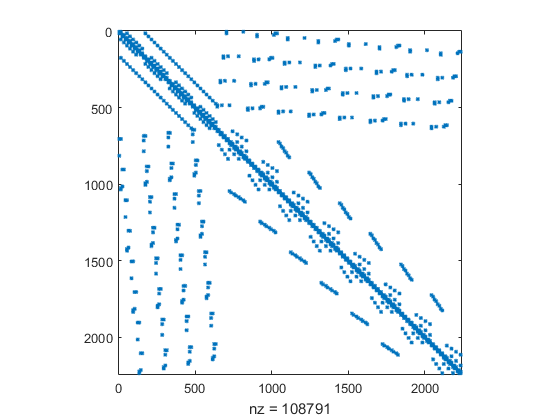
\includegraphics[scale=0.8]{spy_A}
	\caption{Sparsity pattern of $\mathrm{A}$ computed over a mesh of 392 
	polyhedral elements and $r=2$, number of non zero entries (nz) is 271192.}
	\label{fig:spy}
\end{figure}
\newline
For what concerns the right hand side $\mathbf{f}$ we have three contributions:
\begin{equation*}
\mathbf{f} = \mathbf{f}_\mathrm{V} - \mathbf{f}_\mathrm{I} + \mathbf{f}_\mathrm{S},
\end{equation*}
where
\begin{equation*}
	\mathbf{f}_{\mathrm{V}, i} = \sum_{\kappa \in \mathcal{T}} \int_\kappa f \phi_i, \quad
	\mathbf{f}_{\mathrm{I}, i} = \sum_{e \in \Gamma_D} \int_e g (\nabla \phi_i \cdot \mathbf{n}), \quad
	\mathbf{f}_{\mathrm{S}, i} = \sum_{e \in \Gamma_D} \gamma_e \int_e g \phi_i,
	\quad i = 1,\dots,N_h.
\end{equation*}
%%%%%%%%%%%%%%%%%%%%%%%%%%%%%%%%%%%%%%%%%%%%%%%%%%%%%%%%%%%%%%%%%%%%%%%%%
\subsection{Quadrature rules}
Quadrature over general polyhedral elements and polygonal faces is undertaken 
on first constructing a sub-triangulation, followed by the exploitation of 
standard integration schemes. For every polyhedral element $\kappa \in 
\mathcal{T}$ we first construct a non-overlapping sub-triangulation 
$\kappa_\mathcal{S} = \{\tau_\kappa\}$ made of tetrahedral elements, then we 
map quadrature nodes from a reference simplex to each tetrahedron 
$\tau_\kappa$. For example considering the first term of the bilinear form 
$a(\cdot, \cdot)$:
\begin{equation*}
	\int_\kappa \nabla u \cdot \nabla v = \sum_{\tau_\kappa \in \kappa_\mathcal{S}} \nabla u \cdot \nabla v \approx \sum_{\tau_\kappa \in \kappa_\mathcal{S}} \sum_{i=1}^{q} \nabla u(F_\kappa(\xi_i)) \cdot \nabla v(F_\kappa(\xi_i)) det(J_{F_\kappa}(\xi_i))w_i,
\end{equation*}
where $F_\kappa: \hat{\kappa} \rightarrow \tau_\kappa$ is the map from the 
reference simplex $\hat{\kappa}$ to $\tau_\kappa$, $J_{F_\kappa}$ is its 
Jacobian	and $(\xi_i, w_i)^q_{i=1}$ denote the quadrature nodes and weights 
over $\hat{\kappa}$. Observe that the gradient operator is not transformed, as 
it happens when integrals are computer on the reference simplex.\\
Integrals over faces of polyhedral elements can be computed in an analogous 
manner, mapping quadrature points from a reference triangle to each triangular 
face. Of course it is useful for the implementation if each face of a 
polyhedron $\kappa$ coincide with a face of a tetrahedron $\tau_\kappa$ of the 
sub-triangulation $\kappa_\mathcal{S}$.
%%%%%%%%%%%%%%%%%%%%%%%%%%%%%%%%%%%%%%%%%%%%%%%%%%%%%%%%%%%%%%%%%%%%%%%%%
\subsection{Mesh structures}
In our implementation we chose to generate polyhedral meshes by agglomerating 
tetrahedral elements using the software 
METIS\footnote{\url{http://glaros.dtc.umn.edu/gkhome/metis/metis/overview}}. It 
converts the mesh into either a \textit{dual graph} (i.e. each element becomes 
a graph node) or a \textit{nodal graph} (i.e. each vertex becomes a graph 
node), then it partitions it in a given number of portions based on employing 
either a \textit{multilevel recursive bisection} or a \textit{multilevel k-way} 
partitioning algorithm. We intend each portion to be a polyhedral element of 
our mesh and METIS gives us the list of tetrahedra it is composed by. Using 
this approach it follows that for every element $\kappa \in \mathcal{T}$ the 
sub-triangulation $\kappa_\mathcal{S}$ required by quadrature rules is already 
available.
%%%%%%%%%%%%%%%%%%%%%%%%%%%%%%%%%%%%%%%%%%%%%%%%%%%%%%%%%%%%%%%%%%%%%%%%%	
\section{Numerical results}\label{sec:res}
We solve problem~\eqref{eq:dgfempolyform} on the unit cube $\Omega = (0,1)^3$, 
using different kinds of meshes and analysing the asymptotic behaviour of the 
method that we presented. We choose the source term $f$ and the Dirichlet datum 
$g$ such that the exact solution is given by:
\begin{equation*}
	u(x,y,z) = e^{xyz}.
\end{equation*}
We set the penalty constant $\sigma$ defined in \eqref{eq:penalty} equal to 10.\\
Denoting the numerical error by $e_h= u - u_h$, we compute for each mesh the 
$H^1$-seminorm $|\!| \nabla e_h |\!|_{L^2(\mathcal{T})}$, which is bounded 
above by the $DG$-norm, and the $L^2$-norm $|\!|e_h|\!|_{L^2(\mathcal{T})}$.
%%%%%%%%%%%%%%%%%%%%%%%%%%%%%%%%%%%%%%%%%%%%%%%%%%%%%%%%%%%%%%%%%%%%%%%%%%
\subsection{\textit{h}-convergence}
First we solve problem~\eqref{eq:dgfempolyform} over four structured 
tetrahedral meshes of 48, 
384, 1296 and 3072 elements, for $r=1,2,3$. We see in Table~\ref{tab:htet} that 
convergence rates with respect to $h$-convergence are optimal: they correspond 
to theoretical ones given by the estimates~\eqref{eq:dgbound} 
and~\eqref{eq:l2bound}.\\
\begin{table}[h]\footnotesize
	\centering
	\[
	\begin{array}{ccccccc}
	\toprule
	r & Error & \text{48 elem} & \text{384 elem} & \text{1296 elem} & \text{3072 elem} & \text{Rate} \\ 
	\midrule
	1 & |\!|\nabla e_{h}|\!|_{L^2}   & 3.7594 \times 10^{-1} & 1.9785 \times 10^{-1} & 1.3266 \times 10^{-1} & 9.9471 \times 10^{-2} & 1.0009\\
	& |\!|e_{h}|\!|_{L^2} & 1.1256 \times 10^{-2} & 3.6017 \times 10^{-3} & 1.7376 \times 10^{-3} & 1.0227 \times 10^{-3} & 1.8426\\
	\midrule
	2 & |\!|\nabla e_{h}|\!|_{L^2}   & 6.5447 \times 10^{-2} & 1.7846 \times 10^{-2} & 8.1377 \times 10^{-3} & 4.6327 \times 10^{-3} & 1.9583\\
	& |\!|e_{h}|\!|_{L^2} & 5.3216 \times 10^{-3} & 7.2800 \times 10^{-4} & 2.2107 \times 10^{-4} & 9.4460 \times 10^{-5} & 2.9557\\
	\midrule
	3 & |\!|\nabla e_{h}|\!|_{L^2}   & 1.1484 \times 10^{-2} & 1.5987 \times 10^{-3} & 4.8485 \times 10^{-4} & 2.0627 \times 10^{-4} & 2.9708\\
	& |\!|e_{h}|\!|_{L^2} & 8.3358 \times 10^{-4} & 5.7744 \times 10^{-5} & 1.1575 \times 10^{-5} & 3.6715 \times 10^{-6} & 3.9915\\
	\bottomrule
	\end{array}
	\]
	\caption{Computed errors on a sequence of tetrahedral meshes consisting of 
	48, 384, 1296, 3072 elements and polynomial degree $r=1,2,3$.} \label{tab:htet}
\end{table}
Next, we move to structured hexahedral meshes: we consider a sequence of four 
meshes consisting of 8, 64, 216, 512 elements. We see in 
Table~\ref{tab:hhex} that again we obtain convergence rates that are in 
agreement with the estimates of Theorem~\ref{teo:convergence}.\\
Next, we test a sequence of mixed meshes, made of both tetrahedral and 
hexahedral elements. The results are reported in Table~\ref{tab:hhextet} and 
again optimal convergence rates are obtained.\\
The last set of experiments have been carried out over general polyhedral 
meshes generated with METIS, in which different kinds of polyhedra are 
employed. In Table~\ref{tab:hpol} we observe that, even if the rates are not 
perfect since meshes are no more well structured, our DG polyhedral method can 
manage successfully.
\begin{table}[h!]\footnotesize
	\centering
	\[
	\begin{array}{ccccccc}
	\toprule
	r & Error & \text{8 elem} & \text{64 elem} & \text{216 elem} & 
	\text{512 elem} & \text{Rate} \\ 
	\midrule
	1 & |\!|\nabla e_{h}|\!|_{L^2} & 3.1840 \times 10^{-1} & 1.6678 \times 
	10^{-1} & 1.1196 \times 10^{-1} & 8.4123 \times 10^{-2} & 0.9938\\
	& |\!|e_{h}|\!|_{L^2} & 2.7755 \times 10^{-2} & 7.3256 \times 10^{-3} & 3.3204 \times 10^{-3} & 
	1.8931 \times 10^{-3} & 1.9530\\
	\midrule
	2 & |\!|\nabla e_{h}|\!|_{L^2} & 6.9691 \times 10^{-2} & 1.8519 \times 
	10^{-2} & 8.2554 \times 10^{-3} & 4.6362 \times 10^{-3} & 2.0056\\
	& |\!|e_{h}|\!|_{L^2} & 4.9882 \times 10^{-3} & 6.5314 \times 10^{-4} & 1.9059 \times 10^{-4} & 
	7.9122 \times 10^{-5} & 3.0560\\
	\midrule
	3 & |\!|\nabla e_{h}|\!|_{L^2} & 1.6100 \times 10^{-2} & 2.1286 \times 
	10^{-3} & 6.1836 \times 10^{-4} & 2.5782 \times 10^{-4} & 3.0409\\
	& |\!|e_{h}|\!|_{L^2} & 1.0479 \times 10^{-3} & 6.6445 \times 10^{-5} & 1.2080 \times 10^{-5} & 
	3.6604 \times 10^{-6} & 4.1503\\
	\bottomrule
	\end{array}
	\]
	\caption{Computed errors on a sequence of hexahedral meshes consisting of 
		8, 64, 216, 512 elements and polynomial degree $r=1,2,3$.} \label{tab:hhex}
%\end{table}
%\begin{table}[h]\footnotesize
%	\centering
	\[
	\begin{array}{ccccccc}
	\toprule
	r & Error & \text{28 elem} & \text{224 elem} & \text{756 elem} & 
	\text{1792 elem} & \text{Rate} \\ 
	\midrule
	1 & |\!|\nabla e_{h}|\!|_{L^2} & 3.3681 \times 10^{-1} & 1.8227 \times 
	10^{-1} & 1.2424 \times 10^{-1} & 9.4090 \times 10^{-2} & 0.9662\\
	& |\!|e_{h}|\!|_{L^2} & 2.5401 \times 10^{-2} & 6.1132 \times 10^{-3} & 2.6651 \times 10^{-3} & 
	1.4851 \times 10^{-3} & 2.0326\\
	\midrule
	2 & |\!|\nabla e_{h}|\!|_{L^2} & 7.4183 \times 10^{-2} & 1.9944 \times 
	10^{-2} & 8.9959 \times 10^{-3} & 5.0984 \times 10^{-3} & 1.9738\\
	& |\!|e_{h}|\!|_{L^2} & 4.1276 \times 10^{-3} & 7.0478 \times 10^{-4} & 2.1079 \times 10^{-4} & 
	8.9470 \times 10^{-5} & 2.9787\\
	\midrule
	3 & |\!|\nabla e_{h}|\!|_{L^2} & 1.8013 \times 10^{-2} & 2.3198 \times 
	10^{-3} & 6.6815 \times 10^{-4} & 2.7689 \times 10^{-4} & 3.0621\\
	& |\!|e_{h}|\!|_{L^2} & 1.1527 \times 10^{-3} & 7.1514 \times 10^{-5} & 1.3122 \times 10^{-5} & 
	3.9958 \times 10^{-6} & 4.1332\\
	\bottomrule
	\end{array}
	\]
	\caption{Computed errors on a sequence of mixed tetrahedral/hexahedral 
	meshes consisting of 28, 224, 756, 1792 elements and polynomial degree 
	$r=1,2,3$.} \label{tab:hhextet}
%\end{table}
%\begin{table}[h]\footnotesize
%	\centering
	\[
	\begin{array}{ccccccc}
	\toprule
	r & Error & \text{15 elem} & \text{120 elem} & \text{392 elem} & 
	\text{965 elem} & \text{Rate} \\ 
	\midrule
	1 & |\!|\nabla e_{h}|\!|_{L^2} & 3.5875 \times 10^{-1} & 2.5131 \times 
	10^{-1} & 1.8462 \times 10^{-1} & 1.4168 \times 10^{-1} & 0.9200\\
	& |\!|e_{h}|\!|_{L^2} & 3.1209 \times 10^{-2} & 1.7716 \times 10^{-2} & 1.0018 \times 10^{-2} & 
	5.9973 \times 10^{-3} & 1.7935\\
	\midrule
	2 & |\!|\nabla e_{h}|\!|_{L^2} & 8.7963 \times 10^{-2} & 4.2298 \times 
	10^{-2} & 2.3058 \times 10^{-2} & 1.3036 \times 10^{-2} & 1.9823\\
	& |\!|e_{h}|\!|_{L^2} & 5.3520 \times 10^{-3} & 1.8324 \times 10^{-3} & 7.5865 \times 10^{-4} & 2.8963 \times 10^{-4} & 3.3472\\
	\midrule
	3 & |\!|\nabla e_{h}|\!|_{L^2} & 1.9945 \times 10^{-2} & 6.1835 \times 
	10^{-3} & 2.5932 \times 10^{-3} & 1.1137 \times 10^{-3} & 2.9381\\
	& |\!|e_{h}|\!|_{L^2} & 1.4164 \times 10^{-3} & 2.2474 \times 10^{-4} & 7.0145 \times 10^{-5} & 2.0407 \times 10^{-5} & 4.2918\\
	\bottomrule
	\end{array}
	\]
	\caption{Computed errors on a sequence of polyhedral meshes consisting of 
	15, 120, 392, 965 elements and polynomial degree $r=1,2,3$.} \label{tab:hpol}
\end{table}
\begin{figure}[p] 
	\centering
	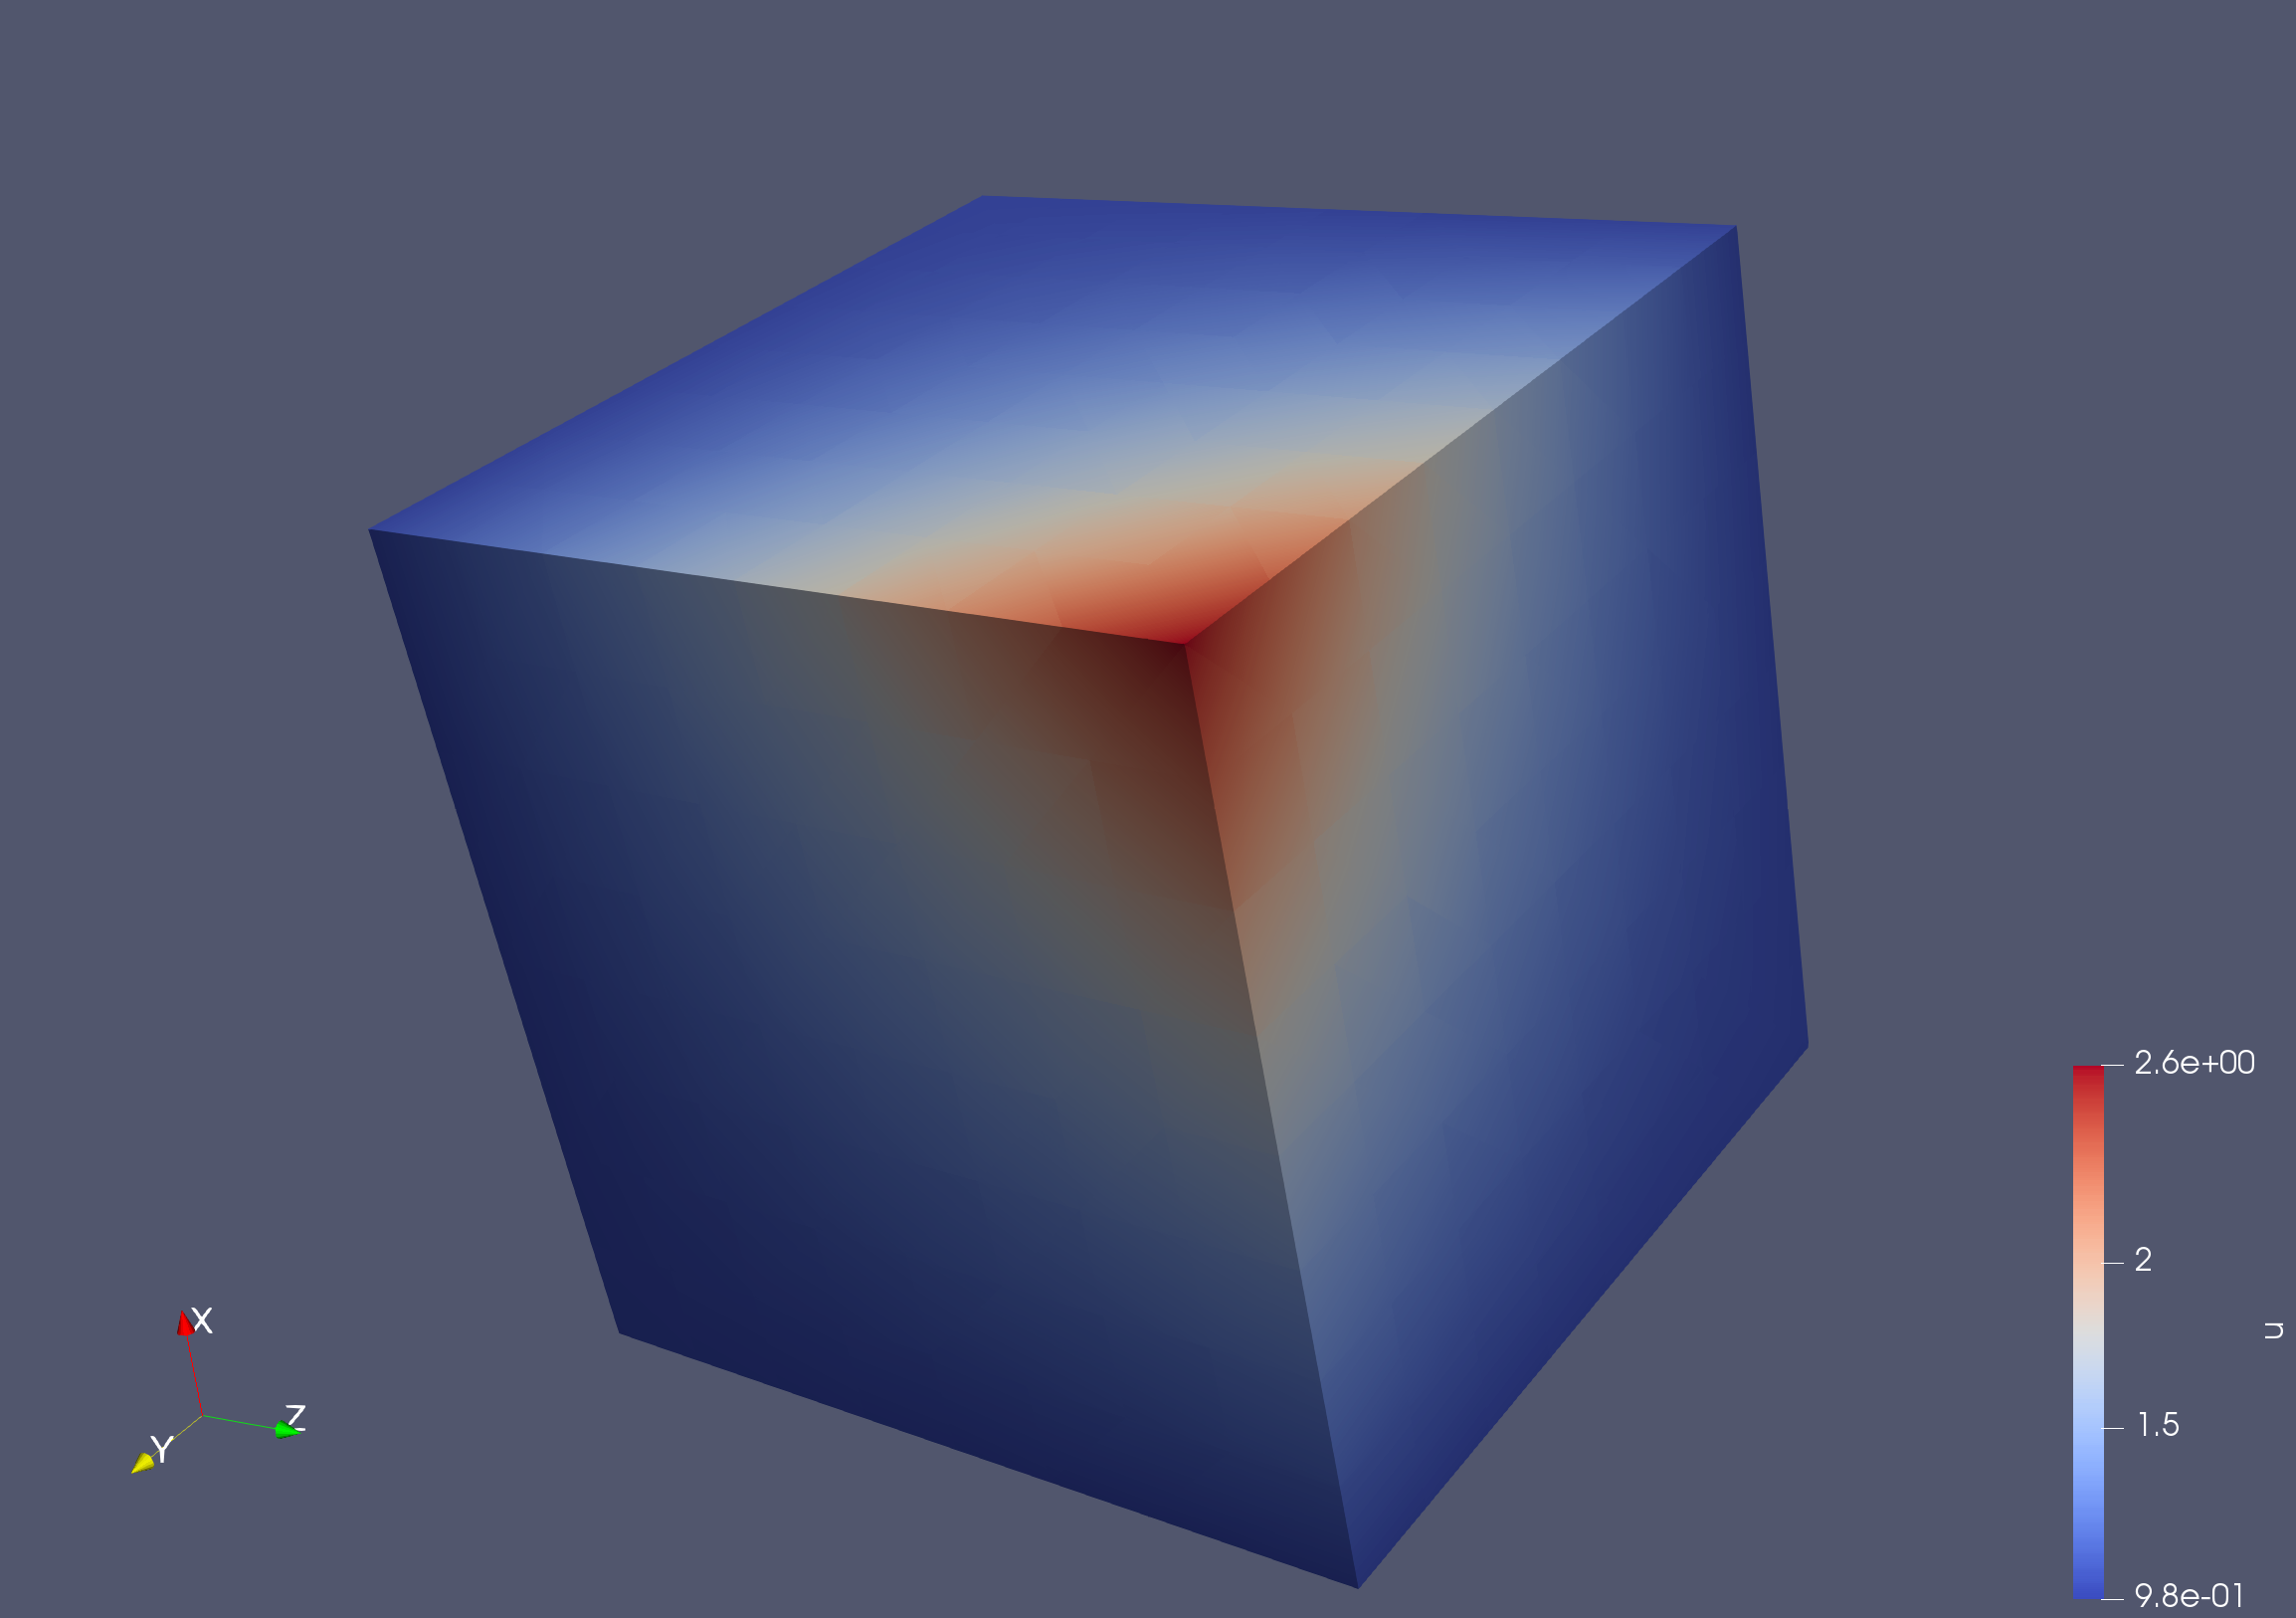
\includegraphics[scale=0.15]{solution_3072p}
	\caption{Solution of the problem~\eqref{eq:dgfempolyform} on the unit cube $\Omega = (0,1)^3$, with $f$ and $g$ such that the exact solution is $u(x,y,z)=e^{xyz}$, $\sigma=10$, employing a polyhedral mesh consisting of 965 elements.}
	\label{fig:sol}
\end{figure}
\begin{figure}[p]
	\centering
	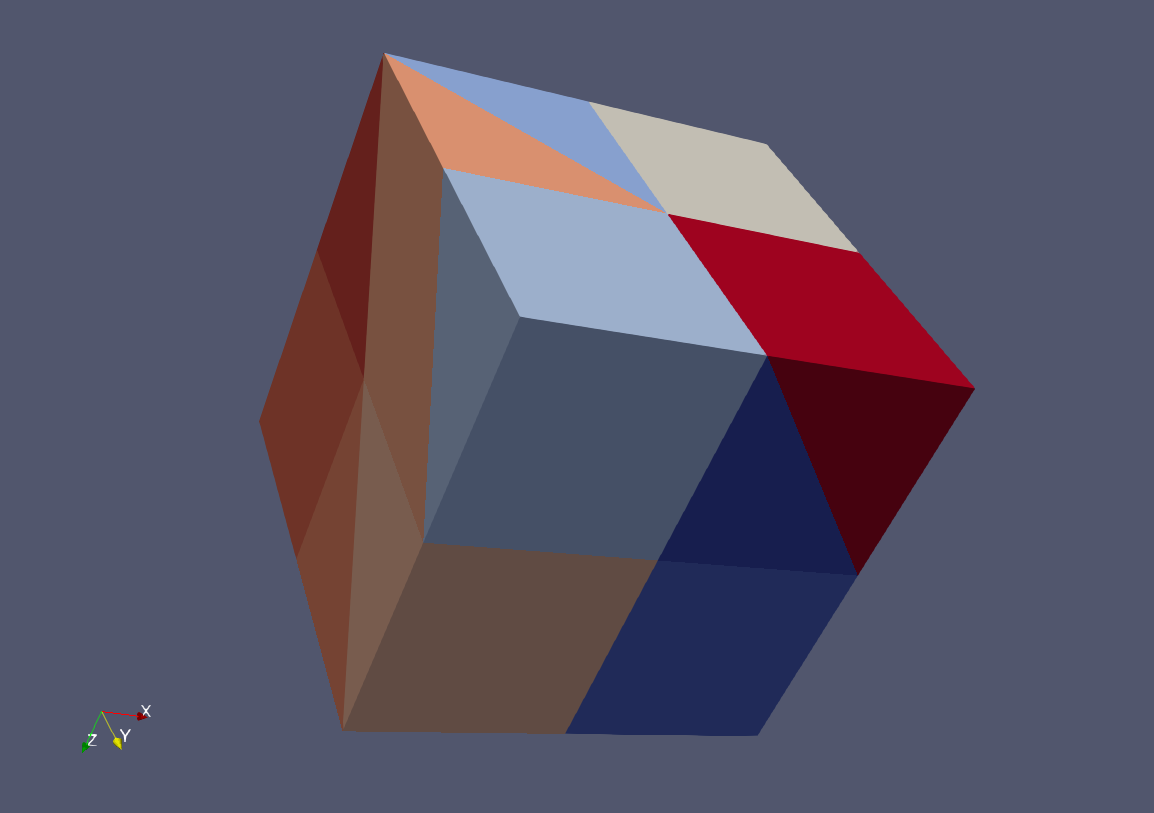
\includegraphics[scale=0.30]{mesh_48p}
	\caption{Polyhedral mesh consisting of 15 elements.}
	\label{fig:mesh}
\end{figure}
%%%%%%%%%%%%%%%%%%%%%%%%%%%%%%%%%%%%%%%%%%%%%%%%%%%%%%%%%%%%%%%%%%%%%%%%%%%%%
\subsection{Comparison with other finite element methods}
We next compare our DG method on polyhedral meshes with the classical SIPG 
method~\eqref{eq:dgfemform}, based on a Lagrange polynomial basis, and with the 
standard continuous Galerkin finite element method (computed with 
FreeFem++\footnote{\url{http://www.freefem.org/}}). As shown in 
Figure~\ref{fig:comp}, where the computed errors as a function of the diameter 
are shown, DG method over polyhedral meshes outperforms the classical SIPG 
scheme based on Lagrange functions as well as the conforming FEM.
\begin{figure}[h]
\centering
\subfloat[][$r=1$, $|\!|\nabla e_h|\!|_{L^2(\mathcal{T})}$] {
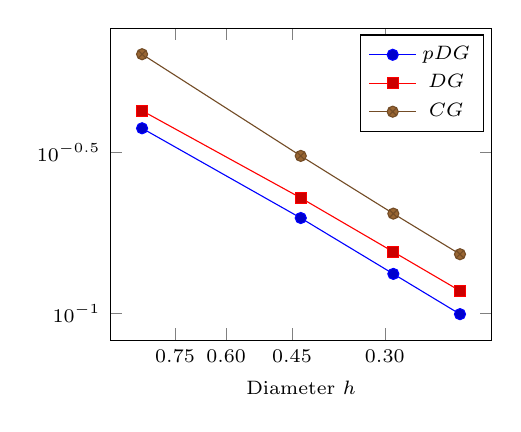
\begin{tikzpicture}
\begin{loglogaxis}[width=0.53\textwidth, xlabel=Diameter $h$, x dir=reverse, 
xtick={0.30,0.45,0.60, 0.75}, xticklabels={$0.30$,$0.45$,$0.60$,$0.75$}]
\addplot coordinates
{(0.866, 3.7594e-1) (0.433, 1.9785e-1) (0.289, 1.3266e-1) (0.216, 9.9471e-2)};
\addlegendentry{$pDG$}
\addplot coordinates
{(0.866, 4.2617e-1) (0.433, 2.2842e-1) (0.289, 1.5530e-1) (0.216, 1.1752e-1)};
\addlegendentry{$DG$}
\addplot coordinates
{(0.866, 6.3842e-1) (0.433, 3.0849e-1) (0.289, 2.0414e-1) (0.216, 1.5270e-1)};
\addlegendentry{$CG$}
%\begin{loglogaxis}[width=0.53\textwidth, xlabel=dof]
%\addplot coordinates
%{(192, 3.7594e-1) (1536, 1.9785e-1) (5184, 1.3266e-1) (12288, 9.9471e-2)};
%\addlegendentry{$pDG$}
%\addplot coordinates
%{(192, 4.2617e-1) (1536, 2.2842e-1) (5184, 1.5530e-1) (12288, 1.1752e-1)};
%\addlegendentry{$DG$}
%\addplot coordinates
%{(27, 6.3842e-1) (125, 3.0849e-1) (343, 2.0414e-1) (729, 1.5270e-1)};
%\addlegendentry{$CG$}
%\legend{$pDG$, $DG$, $CG$}
\end{loglogaxis}
\end{tikzpicture}}
\subfloat[$r=1$, $|\!|e_h|\!|_{L^2(\mathcal{T})}$]{
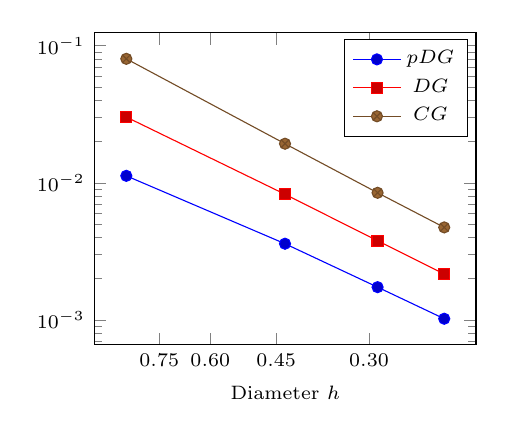
\begin{tikzpicture}
\begin{loglogaxis}[width=0.53\textwidth, xlabel=Diameter $h$, x dir=reverse, xtick={0.30,0.45,0.60, 0.75}, xticklabels={$0.30$,$0.45$,$0.60$,$0.75$}]
\addplot coordinates
{(0.866, 1.1256e-2) (0.433, 3.6017e-3) (0.289, 1.7376e-3) (0.216, 1.0227e-3)};
\addlegendentry{$pDG$}
\addplot coordinates
{(0.866, 3.0189e-2) (0.433, 8.2593e-3) (0.289, 3.7849e-3) (0.216, 2.1654e-3)};
\addlegendentry{$DG$}
\addplot coordinates
{(0.866, 8.0221e-2) (0.433, 1.9297e-2) (0.289, 8.4678e-3) (0.216, 4.7368e-3)};
\addlegendentry{$CG$}
%\legend{$pDG$, $DG$, $CG$}
\end{loglogaxis}
\end{tikzpicture}}\\
\subfloat[][$r=2$, $|\!|\nabla e_h|\!|_{L^2(\mathcal{T})}$]{
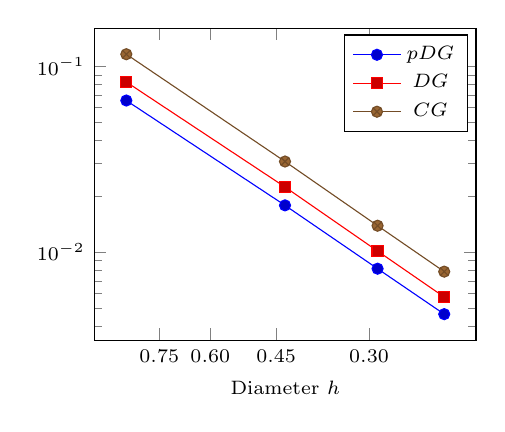
\begin{tikzpicture}
\begin{loglogaxis}[width=0.53\textwidth, xlabel=Diameter $h$, x dir=reverse, xtick={0.30,0.45,0.60, 0.75}, xticklabels={$0.30$,$0.45$,$0.60$,$0.75$}]
\addplot coordinates
{(0.866, 6.5447e-2) (0.433, 1.7846e-2) (0.289, 8.1377e-3) (0.216, 4.6327e-3)};
\addlegendentry{$pDG$}
\addplot coordinates
{(0.866, 8.2336e-2) (0.433, 2.2406e-2) (0.289, 1.0125e-2) (0.216, 5.7278e-3)};
\addlegendentry{$DG$}
\addplot coordinates
{(0.866, 1.1617e-1) (0.433, 3.0729e-2) (0.289, 1.3864e-2) (0.216, 7.8470e-3)};
\addlegendentry{$CG$}
%\legend{$pDG$, $DG$, $CG$}
\end{loglogaxis}
\end{tikzpicture}}
\subfloat[$r=2$, $|\!|e_h|\!|_{L^2(\mathcal{T})}$]{
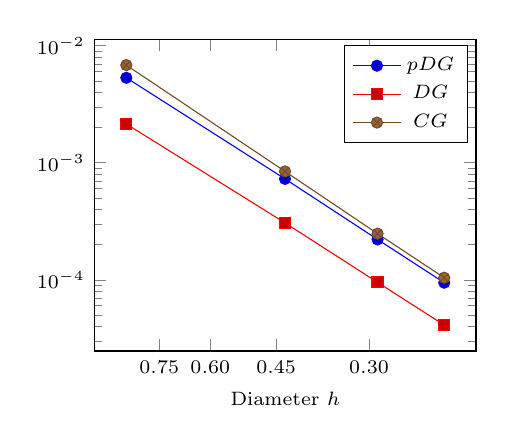
\begin{tikzpicture}
\begin{loglogaxis}[width=0.53\textwidth, xlabel=Diameter $h$, x dir=reverse, xtick={0.30,0.45,0.60, 0.75}, xticklabels={$0.30$,$0.45$,$0.60$,$0.75$}]
\addplot coordinates
{(0.866, 5.3216e-3) (0.433, 7.2800e-4) (0.289, 2.2107e-4) (0.216, 9.4460e-5)};
\addlegendentry{$pDG$}
\addplot coordinates
{(0.866, 2.1435e-3) (0.433, 3.0647e-4) (0.289, 9.5019e-5) (0.216, 4.1058e-5)};
\addlegendentry{$DG$}
\addplot coordinates
{(0.866, 6.8249e-3) (0.433, 8.4316e-4) (0.289, 2.4775e-4) (0.216, 1.0415e-4)};
\addlegendentry{$CG$}
%\legend{$pDG$, $DG$, $CG$}
\end{loglogaxis}
\end{tikzpicture}}
\caption{Computed errors on a sequence of tetrahedral meshes consisting of 48, 
384, 1296, 3072 elements and polynomial degree $r=1,2$. Comparison among 
polyhedral DG method (pDG), classical SIPG method based on Lagrange shape 
functions (DG) and continuous Galerkin finite element method (CG).} 
\label{fig:comp}	
\end{figure}
%%%%%%%%%%%%%%%%%%%%%%%%%%%%%%%%%%%%%%%%%%%%%%%%%%%%%%%%%%%%%%%%%%%%%%%%%%%%%%%
\subsection{\textit{r}-convergence}
Finally we investigate the convergence with respect to $r$-refinement. In 
Figure~\ref{fig:rconv} we report the computed errors as a function of $r$ on a 
grid consisting of tetrahedral, hexahedral, tetrahedral/hexahedral and 
polyhedral elements. As expected we have exponential convergence with every 
kind of mesh since, on the linear-log scale, the convergence plots become 
straight lines.
\begin{figure}[h]
	\centering
	\subfloat[][Tetrahedral elements.]{
	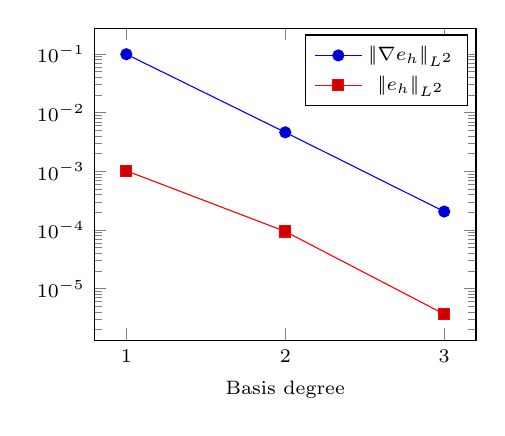
\begin{tikzpicture}
	\begin{semilogyaxis}[width=0.53\textwidth, xlabel={Basis degree}, 
	xtick={1,2,3}]
	\addplot coordinates
	{(1, 9.9471e-2) (2, 4.6327e-3) (3, 2.0627e-4)};
	\addlegendentry{$|\!|\nabla e_{h}|\!|_{L^2}$}	
	\addplot coordinates
	{(1, 1.0227e-3) (2, 9.4460e-5) (3, 3.6715e-6)};
	\addlegendentry{$|\!|e_{h}|\!|_{L^2}$}
%	\legend{$|\!|\nabla e_{h}|\!|_{L^2}$, $|\!|e_{h}|\!|_{L^2}$}
	\end{semilogyaxis}
	\end{tikzpicture}}
	\subfloat[][Hexahedral elements.]{
	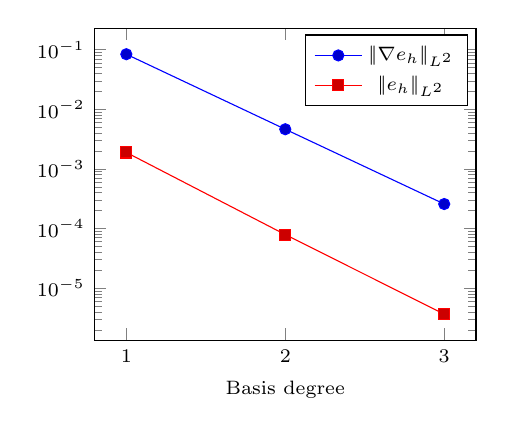
\begin{tikzpicture}
	\begin{semilogyaxis}[width=0.53\textwidth, xlabel={Basis degree}, 
	xtick={1,2,3}]
	\addplot coordinates
	{(1, 8.4123e-2) (2, 4.6362e-3) (3, 2.5782e-4)};
	\addlegendentry{$|\!|\nabla e_{h}|\!|_{L^2}$}	
	\addplot coordinates
	{(1, 1.8931e-3) (2, 7.9122e-5) (3, 3.6604e-6)};
	\addlegendentry{$|\!|e_{h}|\!|_{L^2}$}
%	\legend{$|\!|\nabla e_{h}|\!|_{L^2}$, $|\!|e_{h}|\!|_{L^2}$}
	\end{semilogyaxis}
	\end{tikzpicture}}\\
	\subfloat[][Tetrahedral/hexahedral elements.]{
	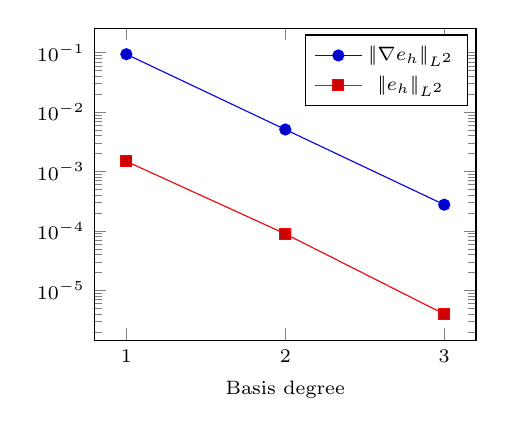
\begin{tikzpicture}
	\begin{semilogyaxis}[width=0.53\textwidth, xlabel={Basis degree}, 
	xtick={1,2,3}]
	\addplot coordinates
	{(1, 9.4090e-2) (2, 5.0984e-3) (3, 2.7689e-4)};
	\addlegendentry{$|\!|\nabla e_{h}|\!|_{L^2}$}	
	\addplot coordinates
	{(1, 1.4851e-3) (2, 8.9470e-5) (3, 3.9958e-6)};
	\addlegendentry{$|\!|e_{h}|\!|_{L^2}$}
%	\legend{$|\!|\nabla e_{h}|\!|_{L^2}$, $|\!|e_{h}|\!|_{L^2}$}
	\end{semilogyaxis}
	\end{tikzpicture}}
	\subfloat[][Polyhedral elements.]{
	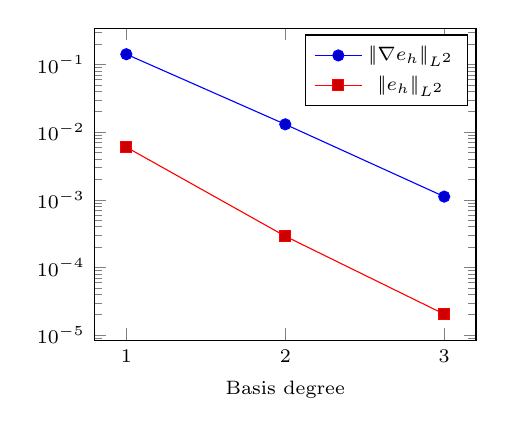
\begin{tikzpicture}
	\begin{semilogyaxis}[width=0.53\textwidth, xlabel={Basis degree}, 
	xtick={1,2,3}]
	\addplot coordinates
	{(1, 1.4168e-1) (2, 1.3036e-2) (3, 1.1137e-3)};
	\addlegendentry{$|\!|\nabla e_{h}|\!|_{L^2}$}	
	\addplot coordinates
	{(1, 5.9973e-3) (2, 2.8963e-4) (3, 2.0407e-5)};
	\addlegendentry{$|\!|e_{h}|\!|_{L^2}$}
	\end{semilogyaxis}
	\end{tikzpicture}}
	\caption{Errors of the DG polyhedral method with respect to $r$-refinement 
	over different kinds of meshes.} \label{fig:rconv}
\end{figure}
%%%%%%%%%%%%%%%%%%%%%%%%%%%%%%%%%%%%%%%%%%%%%%%%%%%%%%%%%%%%%%%%%%%%%%%%%%%%
\section{Conclusions}\label{sec:conc}
We have shown that the DGFEM method on polyhedral meshes that has a great 
flexibility, as it can handle different kinds of meshes always with 
optimal convergence rates. The assumptions on the meshes are weak and do not 
impose any restriction on the number of faces, angles or relative sizes of the 
elemental interfaces. A drawback is obviously the higher computational cost due 
to the fact that the basis is evaluated directly on the 
physical frame and that, as for any DG method, the number of degrees of 
freedom is higher with respect to standard continuous finite elements. This 
issue however can be mitigated by the fact that we can employ fewer elements 
when we have to deal with complicated geometries made of small features or 
microstructures.\\
%We studied only the Poisson problem with Dirichlet boundary conditions, but in 
%future we could expand this algorithm to different boundary conditions without 
%and more complicated elliptic operators without much effort.
%%%%%%%%%%%%%%%%%%%%%%%%%%%%%%%%%%%%%%%%%%%%%%%%%%%%%%%%%%%%%%%%%%%%%%%%%%
\begin{thebibliography}{99}
	\bibitem{review}
	Antonietti P. F., Cangiani  A., Collins J., Dong Z., Georgoulis E. H., Giani S., Houston P.: Review of discontinuous Galerkin finite element methods for partial differential equations on complicated domains. \emph{Building bridges: connections and challenges in modern approaches to numerical partial differential equations, Lecture Notes in Computational Science and Engineering}, volume 114, 279–307 (2016).
	
	\bibitem{mox}
	Antonietti, P. F., Facciolà, C., Russo, A., Verani, M.: Discontinuous Galerkin approximation of flows in fractured porous media on polygonal and polyhedral meshes. \emph{MOX Report} 55/2016 (2016).
	
	\bibitem{multigrid}
	Antonietti P. F., Houston  P., Hu  X., Sarti  M., Verani M.: Multigrid 
	algorithms for hp-version interior penalty discontinuous Galerkin methods 
	on polygonal and polyhedral meshes. \emph{Calcolo}, 1-30 (2017).
	
	\bibitem{arn82}
	Arnold D. N.: An interior penalty finite element method with discontinuous 
	elements. \emph{SIAM Journal on Numerical Analysis}, 19(4), 742-760 (1982).
	
	\bibitem{ayuso}
	Ayuso de Dios B., Brezzi F., Havle O., Marini L.D.: $L^2$-estimates for the 
	DG IIPG-0 scheme. \emph{Numerical Methods in Partial Differential 
	Equations}, 28, 1440-1465 (2012).
	
	\bibitem{hpmet}
	Cangiani A., Georgoulis E. H., Houston P.: Hp-Version discontinuous 
	Galerkin methods on polygonal and polyhedral meshes. \emph{Mathematical 
	Models and Methods in Applied Sciences}, 24(10), 2009-2041 (2014).
	
	\bibitem{dsw}
	Dawson C., Sun S., Wheeler M. F.: Compatible algorithms for coupled flow 
	and transport. \emph{Computer Methods in Applied Mechanics and 
	Engineering}, 193, 2565-2580 (2004).
	
	\bibitem{dunavant}
	Dunavant D.: High degree efficient symmetrical Gaussian quadrature rules 
	for the triangle. \emph{International Journal for Numerical Methods in 
	Engineering}, 21, 1129-1148 (1985).
	
	\bibitem{paper4}
	Giani S., Houston P.: Domain decomposition preconditioners for 
	discontinuous Galerkin discretizations of compressible fluid flows. 
	\emph{Numerical Mathematics: Theory, Methods and Applications}, 7(2), 
	123-128 (2014).
	
	\bibitem{hest}
	Hesthaven J. S., Warburton T.: \emph{Nodal Discontinuous Galerkin Methods: 
	Algorithms, Analysis and Applications}. Springer, Berlin (2007).
	
	\bibitem{quad3d}
	Keast P.: Moderate-degree tetrahedral quadrature formulas. \emph{Computer 
	Methods in Applied Mechanics and Engineering}, 55, 339-348 (1986).
	
	\bibitem{quart}
	Quarteroni A.: \emph{Numerical Models for Differential Problems}. MS\&A, 
	Springer-Verlag Italia, Milan (2014).
	
	\bibitem{riviere}
	Rivière B.: \emph{Discontinuous Galerkin Methods for Solving Elliptic and 
	Parabolic Equations: Theory and Implementation}, volume 35 of 
	\emph{Frontiers in Applied Mathematics}. Society for Industrial and Applied 
	Mathematics (SIAM), Philadelphia, PA (2008).
	
	\bibitem{rwg}
	Rivière B., Wheeler M. F., Girault V.: Improved energy estimates for 
	interior penalty, constrained and discontinuous Galerkin methods for 
	elliptic problems. Part I. \emph{Computational Geosciences}, 3(3-4), 
	337-360 (1999).
	
	\bibitem{salsa}
	Salsa S.: \emph{Partial Differential Equations in Action: From Modelling to 
	Theory}. Springer (2016).

	\bibitem{whe78}
	Wheeler M. F.: An elliptic collocation-finite element method with interior 
	penalties. \emph{SIAM Journal on Numerical Analysis}, 15(1), 152-161 (1978).
\end{thebibliography}

\end{document}